\documentclass{article}

% Idioma
\usepackage[spanish]{babel}

% márgenes y formato
\usepackage[a4paper,top=2cm,bottom=2cm,left=3cm,right=3cm,marginparwidth=1.75cm]{geometry}
\usepackage{parskip}

% Otros paquetes importantes
\usepackage{amsmath}
\usepackage{amssymb}
\usepackage{graphicx}
\usepackage[colorlinks=true, linkcolor=black, urlcolor=blue]{hyperref}

% PARA APUNTES: darkmode
% \usepackage{darkmode}
% \enabledarkmode

% Titulo y autor
\title{Cúbicas a Trozos}
\author{Álvaro Hernández Riquelme}
\date{\today}

\begin{document}

%%%%%%%%%%%%%%%%%%%%%%%%%%%%%%%%%%

\maketitle
\tableofcontents
\newpage

\section{Introducción}

Nuestra función será
\begin{equation}
f(x) = 3x^4 - x^3 - 3x + 1
\end{equation}

con los nodos $x_0 = 0$, $x_1 = 2$.

\subsection{Obtener la cota de error}

Se nos pide obtener la cota de error $|f(x)-H(x)|$ válida para $0<=2<=1$.

Lo primero que haremos sería obtener la cuarta derivada, que, listando cada una, será:

\begin{alignat*}{2}
&f'(x) &&= 12x^3 - 3x^2 - 3 \\
&f''(x) &&= 36x^2 - 6x \\
&f'''(x) &&= 72x - 6 \\
&f^{(4)}(x) &&= 72
\end{alignat*}

Para finalmente, obtener la cota de error con la formula del pdf, siendo la ecuación $16$:

\begin{equation}
|f(x) - H(x)| \leq C_4 \cdot \frac{h^4}{384}
\end{equation}

Donde $C_4$ es el máximo de la cuarta derivada en el intervalo $[0,2]$, que en este caso es $72$, y h es la distancia entre los nodos, que en este caso es $2$.

Por lo tanto, sustituyendo en la ecuación, tenemos:

\begin{equation}
|f(x) - H(x)| \leq 72 \cdot \frac{2^4}{384}
\end{equation}

\begin{equation}
|f(x) - H(x)| \leq \frac{1152}{384} = 3
\end{equation}

La cota de error es de \boxed{$3$}.

\subsection{Calcular H(x) mediante la Forma de Newton}

En este apartado se nos pide calcular el polinomio de Hermite $H(x)$, por lo que, usaremos las fórmulas vistas en clase, y que se encuentran en el PDF de teoría. Para ello, iremos paso por paso hasta tener todos los valores y poder sustituir en la fórmula de Newton (en el último paso).

Calculamos la primera derivada, necesaria para las diferencias divididas:
$$ f'(x) = \frac{d}{dx}(3x^4 - x^3 - 3x + 1) = 12x^3 - 3x^2 - 3 $$

Evaluamos \(f(x)\) y \(f'(x)\) en los nodos \(a=0\) y \(b=2\):
\begin{itemize}
    \item \(f(0) = 3(0)^4 - (0)^3 - 3(0) + 1 = 1\)
    \item \(f(2) = 3(2)^4 - (2)^3 - 3(2) + 1 = 3(16) - 8 - 6 + 1 = 48 - 8 - 6 + 1 = 35\)
    \item \(f'(0) = 12(0)^3 - 3(0)^2 - 3 = -3\)
    \item \(f'(2) = 12(2)^3 - 3(2)^2 - 3 = 12(8) - 3(4) - 3 = 96 - 12 - 3 = 81\)
\end{itemize}

Los coeficientes del polinomio de Hermite en la forma de Newton son las diferencias divididas \(f[0]\), \(f[0,0]\), \(f[0,0,2]\), y \(f[0,0,2,2]\). Las calculamos según la fórmula ($3$) del PDF de teoría.

\begin{itemize}
    \item \(f[0] = f(0) = 1\)
    \item \(f[0,0] = f'(0) = -3\)
    \item \(f[2] = f(2) = 35\)
    \item \(f[2,2] = f'(2) = 81\)
\end{itemize}

\begin{itemize}
    \item \(f[0,2] = \dfrac{f(2) - f(0)}{2-0} = \dfrac{35 - 1}{2} = \dfrac{34}{2} = 17\)
\end{itemize}

Seguimos con la fórmula mencionada ($3$) del PDF, para las siguientes diferencias divididas, usando valores calculados en las anteriores diferencias:

\begin{itemize}
    \item \(f[0,0,2] = \dfrac{f[0,2] - f[0,0]}{2-0} = \dfrac{17 - (-3)}{2} = \dfrac{20}{2} = 10\)
    \item  \(f[0,2,2] = \dfrac{f[2,2] - f[0,2]}{2-0} = \dfrac{81 - 17}{2} = \dfrac{64}{2} = 32\)
\end{itemize}

Finalmente, con los valores obtenidos, calculamos la última diferencia dividida:

\begin{itemize}
    \item \(f[0,0,2,2] = \dfrac{f[0,2,2] - f[0,0,2]}{2-0} = \dfrac{32 - 10}{2} = \dfrac{22}{2} = 11\)
\end{itemize}

Usando la fórmula de Newton con los nodos \(0,0,2,2\) y los coeficientes calculados:

\begin{equation}
H(x) = f[a] + f[a,a](x-a) + f[a,a,b](x-a)^2 + f[a,a,b,b](x-a)^2(x-b)
\end{equation}
\begin{equation}
H(x) = f[0] + f[0,0](x-0) + f[0,0,2](x-0)(x-0) + f[0,0,2,2](x-0)(x-0)(x-2)
\end{equation}
Sustituyendo los valores de los coeficientes:
\begin{equation}
H(x) = 1 + (-3)x + 10x^2 + 11x^2(x-2)
\end{equation}

Si lo expandimos, la solución finalmente es:

$$ \boxed{H(x) = 11x^3 - 12x^2 - 3x + 1} $$

\subsection{Calcula S(x) resolviendo el sistema de ecuaciones}

Para un único intervalo \([x_0, x_1]\), el polinomio del spline, \(S_0(x)\), se define según la fórmula ($24$) del PDF de la teoría:
\begin{equation}
S_0(x) = \alpha_{0,0} + \alpha_{0,1}(x-x_0) + \alpha_{0,2}(x-x_0)^2 + \alpha_{0,3}(x-x_0)^3
\end{equation}

Necesitamos determinar los cuatro coeficientes \(\alpha_{0,0}, \alpha_{0,1}, \alpha_{0,2}, \alpha_{0,3}\). Para ello, hago sistema de cuatro ecuaciones lineales basado en las siguientes condiciones:

\begin{enumerate}
    \item El spline debe pasar por el punto \((x_0, f(x_0))\). Esto lo saco de la ecuación ($26$) del PDF, que sería:
    $$ \alpha_{0,0} = f(x_0) $$

    \item El spline debe pasar por el punto \((x_1, f(x_1))\). Esto se deriva de la segunda parte de la ecuación ($26$) :
    $$ \alpha_{0,0} + \alpha_{0,1}(x_1-x_0) + \alpha_{0,2}(x_1-x_0)^2 + \alpha_{0,3}(x_1-x_0)^3 = f(x_1) $$

    \item Para un spline natural, la segunda derivada en los extremos del intervalo global es cero. Esto seencuentra en la ecuación ($28$), \(S''(x_0) = 0\). La segunda derivada de \(S_0(x)\) es \(S_0''(x) = 2\alpha_{0,2} + 6\alpha_{0,3}(x-x_0)\). Al evaluar en \(x=x_0\), obtenemos:
    $$ S_0''(x_0) = 2\alpha_{0,2} = 0 \implies \alpha_{0,2} = 0 $$
    Esta es la primera de las ``ecuaciones extra'' mencionadas en la ecuación ($27$).

    \item la ecuación ($28$) exige que \(S''(x_1) = 0\). Al evaluar \(S_0''(x)\) en \(x=x_1\), obtenemos:
    $$ S_0''(x_1) = 2\alpha_{0,2} + 6\alpha_{0,3}(x_1-x_0) = 0 $$
    Esta es la segunda de las ``ecuaciones extra''.
\end{enumerate}


Ahora pasamos a plantear el sistema de ecuaciones.
Primero, evaluamos la función \(f(x) = 3x^4 - x^3 - 3x + 1\) en los nodos \(x_0=0\) y \(x_1=2\):
\begin{itemize}
    \item \(f(0) = 3(0)^4 - (0)^3 - 3(0) + 1 = 1\)
    \item \(f(2) = 3(2)^4 - (2)^3 - 3(2) + 1 = 3(16) - 8 - 6 + 1 = 35\)
\end{itemize}

Ahora, construimos el sistema de 4 ecuaciones con 4 incógnitas (\(\alpha_{0,0}, \alpha_{0,1}, \alpha_{0,2}, \alpha_{0,3}\)) usando las fórmulas deducidas:
\begin{enumerate}
    \item \(\alpha_{0,0} = f(0) = 1\)
    \item \(\alpha_{0,0} + \alpha_{0,1}(2-0) + \alpha_{0,2}(2-0)^2 + \alpha_{0,3}(2-0)^3 = f(2)\) \\
    \(\implies \alpha_{0,0} + 2\alpha_{0,1} + 4\alpha_{0,2} + 8\alpha_{0,3} = 35\)
    \item \(\alpha_{0,2} = 0 \)
    \item \(2\alpha_{0,2} + 6\alpha_{0,3}(2-0) = 0 \implies 2\alpha_{0,2} + 12\alpha_{0,3} = 0\)
\end{enumerate}

Ahora resolveremos por sustitución ya que ya tenemos \(\alpha_{0,2}\) y \(\alpha_{0,0}\):
\begin{itemize}
    \item Sustituimos \(\alpha_{0,2}=0\) :
    \begin{align*}
    &2(0) + 12\alpha_{0,3} = 0 &&\\
    &\alpha_{0,3} = 0 &&
    \end{align*}
    \item Finalmente, sustituimos los valores de \(\alpha_{0,0}\), \(\alpha_{0,2}\) y \(\alpha_{0,3}\):
    \begin{align*}
    &(1) + 2\alpha_{0,1} + 4(0) + 8(0) = 35 &&\\
    &1 + 2\alpha_{0,1} = 35 &&\\
    &2\alpha_{0,1} = 34 &&\\
    &\alpha_{0,1} = 17 &&
    \end{align*}
\end{itemize}
Los coeficientes son: \(\alpha_{0,0} = 1\), \(\alpha_{0,1} = 17\), \(\alpha_{0,2} = 0\), \(\alpha_{0,3} = 0\).

Sustituimos los coeficientes en la fórmula:

$$ S(x) = S_0(x) = \alpha_{0,0} + \alpha_{0,1}(x-x_0) + \alpha_{0,2}(x-x_0)^2 + \alpha_{0,3}(x-x_0)^3 $$
$$ S(x) = 1 + 17(x-0) + 0(x-0)^2 + 0(x-0)^3 $$
$$ \boxed{S(x) = 17x + 1} $$


\subsection{Recalcular el nuevo $H(x)$}

Como $x_2=3>2$, el polinomio $H_0(x)$ en $[0,2]$ permanece inalterado. Sólo hay que construir $H_1(x)$ en el nuevo subintervalo $[2,3]$.

Los nodos (con repeticiones) para $[2,3]$ son: $2,2,3,3$.

Calculamos los valores de la función y su derivada en los nodos:
\begin{align*}
f(2) &= 3\cdot2^4 - 2^3 - 3\cdot2 + 1 = 35, \\
f'(2) &= 12\cdot2^3 - 3\cdot2^2 - 3 = 81, \\
f(3) &= 3\cdot3^4 - 3^3 - 3\cdot3 + 1 = 208, \\
f'(3) &= 12\cdot3^3 - 3\cdot3^2 - 3 = 294.
\end{align*}

Calculamos las diferencias divididas necesarias:
\begin{align*}
f[2] &= 35, \\
f[2,2] &= 81, \\
f[3] &= 208, \\
f[3,3] &= 294, \\
f[2,3] &= \frac{f(3) - f(2)}{3-2} = \frac{208 - 35}{1} = 173, \\
f[2,2,3] &= \frac{f[2,3] - f[2,2]}{3-2} = \frac{173 - 81}{1} = 92, \\
f[2,3,3] &= \frac{f[3,3] - f[2,3]}{3-2} = \frac{294 - 173}{1} = 121, \\
f[2,2,3,3] &= \frac{f[2,3,3] - f[2,2,3]}{3-2} = \frac{121 - 92}{1} = 29.
\end{align*}

Por la fórmula para el polinomio de Hermite en $[2,3]$:
\begin{equation}
H_1(x) = f[2] + f[2,2](x-2) + f[2,2,3](x-2)^2 + f[2,2,3,3](x-2)^2(x-3)
\end{equation}
Sustituyendo los valores obtenidos:
\begin{equation}
H_1(x) = 35 + 81(x-2) + 92(x-2)^2 + 29(x-2)^2(x-3), \quad x \in [2,3].
\end{equation}


Para el $H_0$ tendríamos lo calculado en el primer ejercicio, pues estaba calculado para el intervalo $[0,2]$:

$$ H_0(x) = 11x^3 - 12x^2 - 3x + 1, \quad x \in [0,2]. $$


\subsection{Verificación de la Continuidad de la Función y su Derivada}

Ahora comprobamos si se cumplen las igualdades que se muestran en \eqref{eq:continuity}, que la primera coincidiría con la comprobación de la continuidad en $x=2$ de la función y la segunda la de la derivada.

\begin{equation}
\label{eq:continuity}
\begin{aligned}
H(2^-) &= H(2^+) = f(2) \\
H'(2^-) &= H'(2^+) = f'(2)
\end{aligned}
\end{equation}

La función \(f(x)\) y su derivada \(f'(x)\) las tenemos, y sus valores en el nodo \(x=2\) son:
$$
f(2) = 3(16) - 8 - 6 + 1 = 35
$$
$$
f'(2) = 12(8) - 3(4) - 3 = 96 - 12 - 3 = 81
$$

Ahora calculamos el polinomio a la izquierda, del primer ejercicio tenemos:

$$
H_0(2) = 1 - 3 \cdot 2 + 10 \cdot 2^2 + 11 \cdot 2^2 (2-2) = 1 - 6 + 40 + 0 = 35
$$

Y para la derivada:

$$
H_0'(x)=33x^2-24x-3
$$

$$
H_0'(2)=33\cdot4-48-3=81
$$

Para los coeficientes de la derecha, usamos el polinomio \(H_1(x)\) que hemos calculado en el apartado anterior:

$$H_1(2) = 35+0+0+0 = 35$$

Y la derivada de \(H_1(x)\) es con la regla de la cadena:

$$
H_1'(x)
=81+184(x-2)
+29\Bigl(2(x-2)(x-3)+(x-2)^2\Bigr).
$$

Simplificando,

$$
H_1'(x)=87x^2-222x+177.
$$

Evaluando en \(x=2\):
\[
H_1'(2)=87\cdot2^2-222\cdot2+177
=87\cdot4-444+177
=348-444+177
=81.
\]

Por lo que se cumplen las igualdades


\subsection{Verificación de la Continuidad de la Segunda Derivada}


En este apartado vamos a comprobar si la segunda derivada es continua en el nodo $x=2$.

Primero, calculamos la segunda derivada de $H_0(x)$:

$$
H_0''(x) = 66x - 24.
$$

Evaluando en $x=2$:
$$
H_0''(2) = 66 \cdot 2 - 24 = 108.
$$

Ahora, calculamos la segunda derivada de $H_1(x)$:

$$
H_1''(x) = 174x - 222.
$$

Evaluando en $x=2$:

$$
H_1''(2) = 174 \cdot 2 - 222 = 126.
$$

Por último, recordamos la segunda derivada de la función original:
$$
f''(x) = 36x^2 - 6x,
$$
y evaluamos en $x=2$:
$$
f''(2) = 36 \cdot 2^2 - 6 \cdot 2 = 132.
$$

Por lo tanto, los valores obtenidos son:
$$
H_0''(2) = 108, \qquad H_1''(2) = 126, \qquad f''(2) = 132.
$$

Como se puede observar, no se cumple la continuidad de la segunda derivada en $x=2$, ya que los valores de $H_0''(2)$ y $H_1''(2)$ son distintos. Además, ninguno de ellos coincide con la segunda derivada de la función original en ese punto. Por tanto, concluimos que $H''(x)$ no es continua en $x=2$.
\section{Segunda parte: Nuevo $S(x)$ y comprobaciones con maxima }


Calcularemos ahora de la misma forma que antes el nuevo spline \(S(x)\) con el nodo \(x_2=3\). Lo primero, será formar las ecuaciones necesarias para el nuevo spline, que serán las mismas que antes, pero añadiendo varias con el nuevo nodo.

\subsection{Recalcular el nuevo S(x)}

Al añadir el nodo $x_2=3$, ahora tenemos dos intervalos, $[0, 2]$ y $[2, 3]$, y por lo tanto, el spline $S(x)$ estará compuesto por dos polinomios cúbicos:
\begin{itemize}
    \item $S_0(x)$ en el intervalo $[0, 2]$.
    \item $S_1(x)$ en el intervalo $[2, 3]$.
\end{itemize}

La forma general de cada polinomio, como hemos visto antes según la ecuación (24) del PDF de teoría, es:
$$S_i(x) = \alpha_{i,0} + \alpha_{i,1}(x-x_i) + \alpha_{i,2}(x-x_i)^2 + \alpha_{i,3}(x-x_i)^3$$

Tenemos un total de $4n=8$ coeficientes que determinar, por lo que necesitamos plantear un sistema de 8 ecuaciones. Estas ecuaciones se basan en las condiciones de interpolación , continuidad  y las condiciones de frontera para un spline natural.


Necesitamos los valores de la función $f(x) = 3x^4 - x^3 - 3x + 1$ en los tres nodos, los dos primeros ya los tenemos:
\begin{itemize}
    \item $f(x_0) = 1$
    \item $f(x_1) = 35$
    \item $f(x_2) = f(3) = 208$
\end{itemize}

Recordemos, con las condiciones de antes, que el sistema de 8 ecuaciones se construye a partir de:
\begin{itemize}
    \item \textbf{Condiciones de interpolación (3 ecuaciones)}: El spline debe pasar por todos los nodos.
    \item \textbf{Condiciones de continuidad en el nodo interior $x_1=2$ (3 ecuaciones)}: La función, su primera y su segunda derivada deben ser continuas.
    \item \textbf{Condiciones de frontera del spline natural (2 ecuaciones)}: La segunda derivada es cero en los extremos $x_0$ y $x_2$ ($S''(x_0)=S''(x_n)=0$).
\end{itemize}

Sustituimos los valores de los nodos (\(x_0=0, x_1=2, x_2=3\)) y de la función en las condiciones generales para obtener el sistema lineal:
\begin{enumerate}
    \item \(\alpha_{0,0} = f(0) \implies \alpha_{0,0} = 1\)
    \item \(\alpha_{1,0} = f(2) \implies \alpha_{1,0} = 35\)
    \item \(\alpha_{1,0} + \alpha_{1,1}(3-2) + \alpha_{1,2}(3-2)^2 + \alpha_{1,3}(3-2)^3 = f(3)
          \implies 35 + \alpha_{1,1} + \alpha_{1,2} + \alpha_{1,3} = 208\)
    \item \(\alpha_{0,0} + \alpha_{0,1}(2-0) + \alpha_{0,2}(2-0)^2 + \alpha_{0,3}(2-0)^3 = \alpha_{1,0}
          \implies 1 + 2\alpha_{0,1} + 4\alpha_{0,2} + 8\alpha_{0,3} = 35\)
    \item \(\alpha_{0,1} + 2\alpha_{0,2}(2-0) + 3\alpha_{0,3}(2-0)^2 = \alpha_{1,1}
          \implies \alpha_{0,1} + 4\alpha_{0,2} + 12\alpha_{0,3} = \alpha_{1,1}\)
    \item \(2\alpha_{0,2} + 6\alpha_{0,3}(2-0) = 2\alpha_{1,2}
          \implies \alpha_{0,2} + 6\alpha_{0,3} = \alpha_{1,2}\)
    \item \(2\alpha_{0,2} = 0 \implies \alpha_{0,2} = 0\)
    \item \(2\alpha_{1,2} + 6\alpha_{1,3}(3-2) = 0 \implies \alpha_{1,2} + 3\alpha_{1,3} = 0\)
\end{enumerate}

Ahora resolvemos por el método de Cramer:

Tras conocer \(\alpha_{0,0}=1\), \(\alpha_{1,0}=35\) y \(\alpha_{0,2}=0\), para sacar \(\alpha_{0,1}\) y \(\alpha_{0,3}\) podríamos hacerlo con un sistema de dos ecuaciones, usando la ecuacion numerada 3 de las de antes y la  4:

$$
\begin{cases}
1 + 2\alpha_{0,1} + 8\alpha_{0,3} = 35,\\
35 + \alpha_{0,1} + 16\alpha_{0,3} = 208.
\end{cases}
$$

Y simplificando:

$$
\begin{cases}
\alpha_{0,1} + 4\alpha_{0,3} = 17, \\
\alpha_{0,1} + 16\alpha_{0,3} = 173.
\end{cases}
$$

Calculamos los determinantes sustituyendo con lo que ya tenemos:
$$
D = \begin{vmatrix}
1 & 4 \\
1 & 16
\end{vmatrix}
= 1\cdot16 - 1\cdot4 = 12,
$$
$$
D_{1} = \begin{vmatrix}
17 & 4 \\
173 & 16
\end{vmatrix}
= 17\cdot16 - 4\cdot173 = 272 - 692 = -420,
\quad
D_{2} = \begin{vmatrix}
1 & 17 \\
1 & 173
\end{vmatrix}
= 1\cdot173 - 17\cdot1 = 156.
$$

Por Cramer:
$$
\alpha_{0,1} = \frac{D_{1}}{D} = \frac{-420}{12} = -35,
\quad
\alpha_{0,3} = \frac{D_{2}}{D} = \frac{156}{12} = 13.
$$

Finalmente, encontramos los coeficientes restantes:
\begin{itemize}
    \item \(\alpha_{1,2} = 6\alpha_{0,3} = 6\cdot13 = 78\)
    \item \(\alpha_{1,3} = -2\alpha_{0,3} = -2\cdot13 = -26\)
    \item \(\alpha_{1,1} = \alpha_{0,1} + 12\alpha_{0,3} = -35 + 12\cdot13 = 121\)
\end{itemize}

En conclusión, los coeficientes para el intervalo \([0,2]\) son:
$$
\alpha_{0,0} = 1,\quad \alpha_{0,1} = -35,\quad \alpha_{0,2} = 0,\quad \alpha_{0,3} = 13,
$$
$$
S_{0}(x) = 1 - 35\,(x-0) + 0\,(x-0)^{2} + 13\,(x-0)^{3}.
$$

Que en la base canónica:
$$ \boxed{S_0(x) = 13x^3 - 35x + 1} $$

Los coeficientes para el intervalo $[2, 3]$ son:


$$\alpha_{1,0} = 35, \quad \alpha_{1,1} = 121, \quad \alpha_{1,2} = 78, \quad \alpha_{1,3} = -26$$

$$ S_1(x) = 35 + 121(x-2) + 78(x-2)^2 - 26(x-2)^3 $$
En la base canónica:
\begin{align*}
    S_1(x) &= 35 + 121x - 242 + 78(x^2 - 4x + 4) - 26(x^3 - 6x^2 + 12x - 8) \\
    S_1(x) &= -207 + 121x + 78x^2 - 312x + 312 - 26x^3 + 156x^2 - 312x + 208 \\
\end{align*}

$$\boxed{S_1(x) = -26x^3 + 234x^2 - 503x + 313}$$


En comparación con el escenario de solo dos nodos, donde el spline natural resultaba en una línea recta (\(S(x) = 17x + 1\)), al incluir un tercer nodo, los polinomios que salen \(S_0(x)\) y \(S_1(x)\) se transforman en funciones cúbicas. Esto sucede porque, aunque en el caso de dos nodos el spline natural reduce al máximo la curvatura y produce una recta, las exigencias de continuidad en el nodo intermedio (\(x=2\)) para de tres nodos permiten que los coeficientes cúbicos y cuadráticos tengan valores distintos de cero.


\subsection{Verificación de la Continuidad de S(x) en x=2}

Ahora comprobamos si se cumple la condición de continuidad $S(2^-) = S(2^+) = f(2)$. Para ello, utilizamos los dos polinomios del spline que se unen en $x=2$.

El polinomio a la izquierda del nodo, en el intervalo $[0,2]$, es:
$$ S_0(x) = 13x^3 - 35x + 1 $$

El polinomio a la derecha del nodo, en el intervalo $[2,3]$, es:
$$ S_1(x) = 35 + 121(x-2) + 78(x-2)^2 - 26(x-2)^3 $$

Ahora, evaluamos cada uno en $x=2$:

$$ S(2^-) = S_0(2) = 13(2)^3 - 35(2) + 1 = 13(8) - 70 + 1 = 104 - 70 + 1 = \mathbf{35} $$

$$ S(2^+) = S_1(2) = 35 + 121(2-2) + 78(2-2)^2 - 26(2-2)^3 = 35 + 0 + 0 + 0 = \mathbf{35} $$

El valor de la función original en el nodo es:
$$ f(2) = 3(2)^4 - (2)^3 - 3(2) + 1 = 3(16) - 8 - 6 + 1 = \mathbf{35} $$

Se cumple que $S(2^-) = S(2^+) = f(2) = 35$. Esto verifica que la función del spline cúbico es continua en el nodo interior, como se requiere por su definición.

\subsection{Verificación de la Continuidad de las Derivadas de S(x)}

Por definición, el spline cúbico $S(x)$ debe tener una primera y una segunda derivada continuas en los nodos interiores. Vamos a verificar que esto se cumple en $x=2$ para los polinomios que hemos calculado.


Primero, calculamos las derivadas de $S_0(x)$ y $S_1(x)$:
$$ S'_0(x) = \frac{d}{dx}(13x^3 - 35x + 1) = 39x^2 - 35 $$
$$ S'_1(x) = \frac{d}{dx}\left(35 + 121(x-2) + 78(x-2)^2 - 26(x-2)^3\right) = 121 + 156(x-2) - 78(x-2)^2 $$

Ahora, evaluamos en $x=2$:
$$ S'(2^-) = S'_0(2) = 39(2)^2 - 35 = 39(4) - 35 = 156 - 35 = \mathbf{121} $$
$$ S'(2^+) = S'_1(2) = 121 + 156(2-2) - 78(2-2)^2 = 121 + 0 - 0 = \mathbf{121} $$
Se cumple que $S'(2^-) = S'(2^+)$, por lo que la primera derivada es continua.

\vspace{1cm}


Calculamos las segundas derivadas:
$$ S''_0(x) = \frac{d}{dx}(39x^2 - 35) = 78x $$
$$ S''_1(x) = \frac{d}{dx}\left(121 + 156(x-2) - 78(x-2)^2\right) = 156 - 156(x-2) $$

Evaluamos en $x=2$:
$$ S''(2^-) = S''_0(2) = 78(2) = \mathbf{156} $$
$$ S''(2^+) = S''_1(2) = 156 - 156(2-2) = 156 - 0 = \mathbf{156} $$
También se cumple que $S''(2^-) = S''(2^+)$, confirmando que el spline es de clase $\mathcal{C}^2$ en el nodo interior.



\subsection{Comparación de Derivadas: S(x) vs f(x)}

Ahora investigamos si los valores de las derivadas del spline en el nodo $x=2$ coinciden con los valores de las derivadas de la función original $f(x)$.

Primero, calculamos las derivadas de $f(x) = 3x^4 - x^3 - 3x + 1$:
$$ f'(x) = 12x^3 - 3x^2 - 3 $$
$$ f''(x) = 36x^2 - 6x $$

Evaluamos estas derivadas en $x=2$:
$$ f'(2) = 12(2)^3 - 3(2)^2 - 3 = 96 - 12 - 3 = \mathbf{81} $$
$$ f''(2) = 36(2)^2 - 6(2) = 144 - 12 = \mathbf{132} $$

Ahora comparamos estos valores con los que obtuvimos para el spline en el apartado anterior:

$$ S'(2) = 121 \neq f'(2) = 81 $$
$$ S''(2) = 156 \neq f''(2) = 132 $$

Por lo que las derivadas del spline y de la función original no coinciden en los nodos interiores. Esto es un resultado esperado y una diferencia con la interpolación de Hermite. El spline cúbico no utiliza la información de las derivadas de $f(x)$ para su construcción; en su lugar, garantiza la suavidad de la curva resultante asegurando que sus propias derivadas ($S', S''$) sean continuas.

\subsection{Dibuja juntos $S(x)$ y $H(x)$ con Maxima}

Usaremos la función proporcionada en el aula virtual llamada \verb|ComparaCubicas()| en Maxima, a continuación se muestra una captura con los tres nodos y otra con los cuatro nodos.

\begin{figure}[ht]
    \centering
    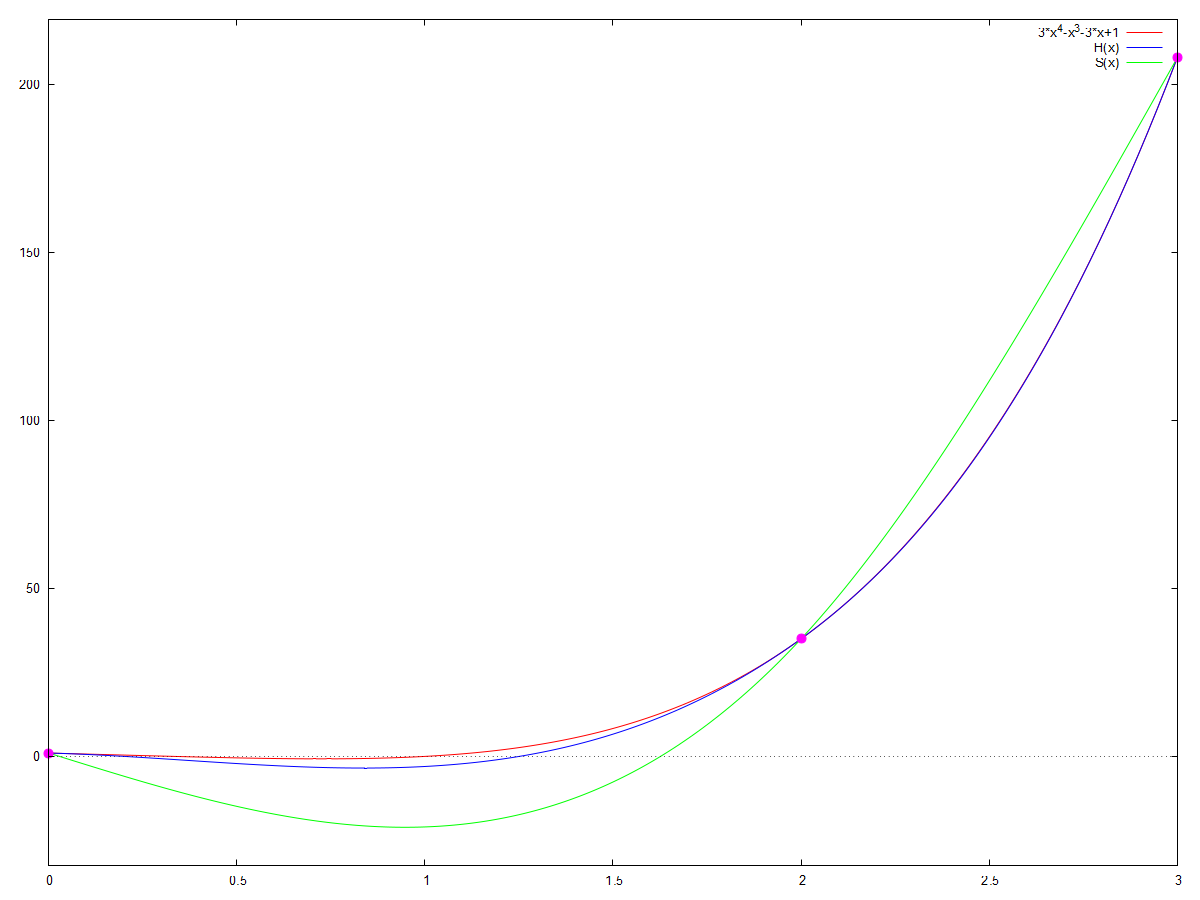
\includegraphics[width=0.7\textwidth]{src/comparacubicas.png}
    \caption{Comparación de $S(x)$ y $H(x)$ con tres nodos}
    \label{fig:tres_nodos}
\end{figure}

\newpage

\begin{figure}[hb]
    \centering
    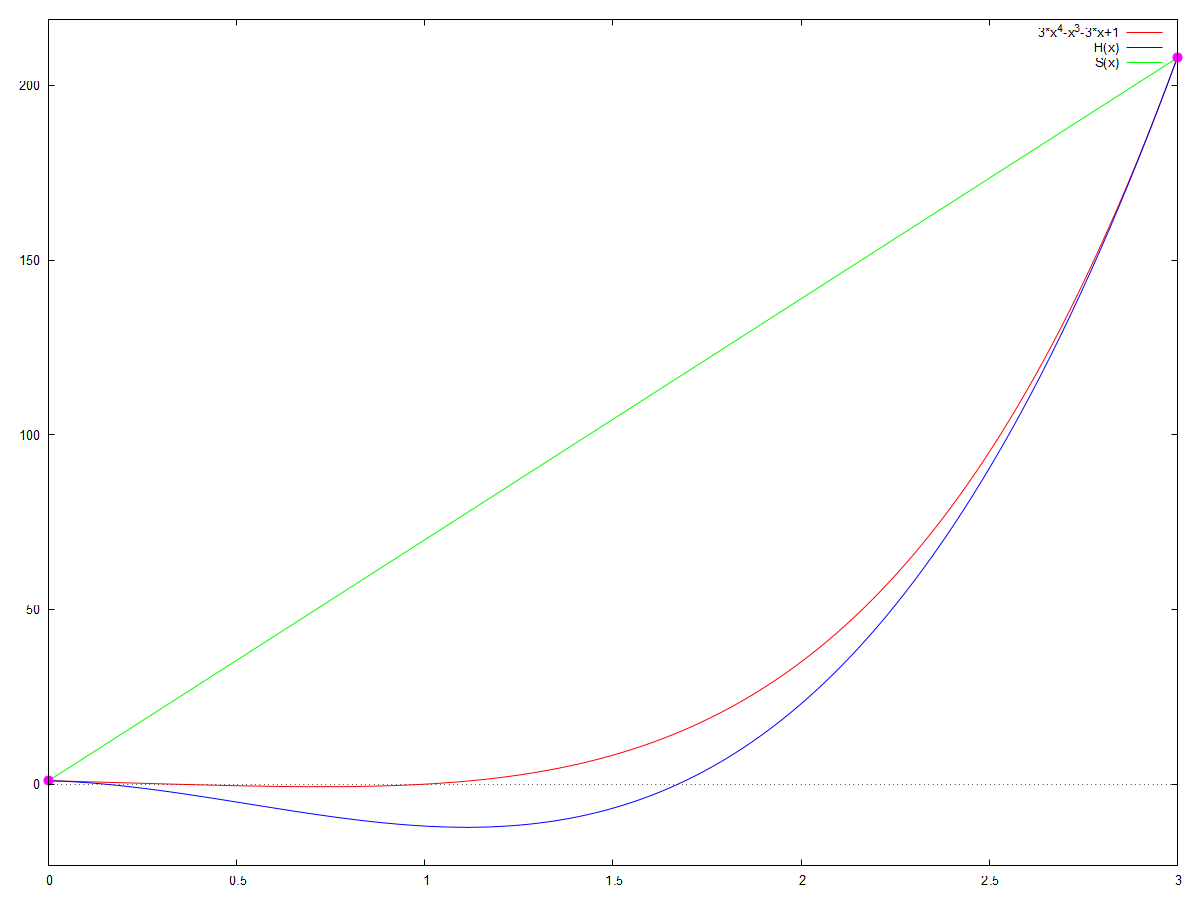
\includegraphics[width=0.7\textwidth]{src/comparacubicas2.png}
    \caption{Comparación de $S(x)$ y $H(x)$ con cuatro nodos}
    \label{fig:cuatro_nodos}
\end{figure}

\newpage

\subsection{Planteamiento del nuevo H(x) con el nodo $x^*=1$}

Al añadir el nodo $x^*=1$ al conjunto existente $\{0, 2, 3\}$, el nuevo conjunto de nodos ordenado es $\{0, 1, 2, 3\}$. Esto divide el problema en tres intervalos: $[0,1]$, $[1,2]$ y $[2,3]$.

La interpolación cúbica a trozos de Hermite posee permanencia. Esto significa que, al añadir un nuevo nodo, únicamente se ven afectados los cálculos del intervalo que contiene dicho nodo; los polinomios en los demás intervalos permanecen inalterados.

El nuevo nodo $x^*=1$ se encuentra dentro del intervalo original $[0,2]$. Según la teoría, ``Todos los cálculos realizados con anterioridad son válidos excepto justamente el de este subintervalo''.

Por lo tanto, si analizamos lo que perdemos y lo que mantenemos:
\begin{itemize}
    \item \textbf{Se pierde:} El polinomio $H_0(x)$ que habíamos calculado para el intervalo $[0,2]$ ya no es válido.
    \item \textbf{Se mantiene:} El polinomio $H_1(x)$ calculado para el intervalo $[2,3]$ sigue siendo válido, ya que su intervalo de definición no ha sido alterado.
    \item \textbf{Se debe calcular:} Debemos construir dos nuevos polinomios cúbicos de Hermite: uno para el nuevo intervalo $[0,1]$ y otro para $[1,2]$.
\end{itemize}

$H(x)$ completo quedaría definido así:
$$ H(x) = \begin{cases} H_{nuevo,0}(x) & \text{si } x \in [0,1] \\ H_{nuevo,1}(x) & \text{si } x \in [1,2] \\ H_1(x) & \text{si } x \in [2,3] \end{cases} $$
donde $H_1(x)$ es el polinomio para el intervalo $[2,3]$ que ya se tenía.


\subsection{Planteamiento del sistema para el nuevo spline S(x)}

A diferencia de la interpolación de Hermite, ``los splines no poseen propiedades de tipo permanencia, de manera que añadir nodos obliga a recalcular todos los coeficientes''.

Con el nuevo conjunto de nodos $\{0, 1, 2, 3\}$, tenemos $n=3$ intervalos, lo que da lugar a 3 polinomios cúbicos:
\begin{itemize}
    \item $S_0(x)$ en $[0,1]$
    \item $S_1(x)$ en $[1,2]$
    \item $S_2(x)$ en $[2,3]$
\end{itemize}

Cada polinomio $S_i(x) = \alpha_{i,0} + \alpha_{i,1}(x-x_i) + \alpha_{i,2}(x-x_i)^2 + \alpha_{i,3}(x-x_i)^3$ tiene 4 coeficientes. Esto nos da un total de $3 \times 4 = 12$ incógnitas. Por tanto, necesitamos plantear un sistema con 12 ecuaciones.

Planteamiento del sistema de 12 ecuaciones

Las ecuaciones se derivan de las condiciones que hemos estado usando hasta ahora:
\begin{itemize}
    \item \textbf{4 Ecuaciones de Interpolación}: El spline debe pasar por los 4 nodos ($S(x_i)=f(x_i)$).
    \item \textbf{6 Ecuaciones de Continuidad}: La función, la primera derivada y la segunda derivada deben ser continuas en los 2 nodos interiores ($x_1=1$ y $x_2=2$).
    \item \textbf{2 Ecuaciones de Frontera (Spline Natural)}: La segunda derivada es nula en los extremos $x_0=0$ y $x_3=3$ ($S''(x_0)=S''(x_n)=0$).
\end{itemize}

Finalmente, el sistema completo es:

\begin{enumerate}
    % Interpolación
    \item $S_0(0) = f(0) \implies \alpha_{0,0} = f(0)$
    \item $S_1(1) = f(1) \implies \alpha_{1,0} = f(1)$
    \item $S_2(2) = f(2) \implies \alpha_{2,0} = f(2)$
    \item $S_2(3) = f(3) \implies \alpha_{2,0} + \alpha_{2,1}(3-2) + \alpha_{2,2}(3-2)^2 + \alpha_{2,3}(3-2)^3 = f(3)$
    % Continuidad en x=1
    \item $S_0(1) = S_1(1) \implies \alpha_{0,0} + \alpha_{0,1}(1-0) + \alpha_{0,2}(1-0)^2 + \alpha_{0,3}(1-0)^3 = \alpha_{1,0}$
    \item $S'_0(1) = S'_1(1) \implies \alpha_{0,1} + 2\alpha_{0,2}(1-0) + 3\alpha_{0,3}(1-0)^2 = \alpha_{1,1}$
    \item $S''_0(1) = S''_1(1) \implies 2\alpha_{0,2} + 6\alpha_{0,3}(1-0) = 2\alpha_{1,2}$
    % Continuidad en x=2
    \item $S_1(2) = S_2(2) \implies \alpha_{1,0} + \alpha_{1,1}(2-1) + \alpha_{1,2}(2-1)^2 + \alpha_{1,3}(2-1)^3 = \alpha_{2,0}$
    \item $S'_1(2) = S'_2(2) \implies \alpha_{1,1} + 2\alpha_{1,2}(2-1) + 3\alpha_{1,3}(2-1)^2 = \alpha_{2,1}$
    \item $S''_1(2) = S''_2(2) \implies 2\alpha_{1,2} + 6\alpha_{1,3}(2-1) = 2\alpha_{2,2}$
    % Frontera
    \item $S''_0(0) = 0 \implies 2\alpha_{0,2} = 0$
    \item $S''_2(3) = 0 \implies 2\alpha_{2,2} + 6\alpha_{2,3}(3-2) = 0$
\end{enumerate}

% \vspace{1cm}
% \begin{center}
% \fbox{\parbox{0.8\textwidth}{
% Ambas igualdades se han verificado. Esto demuestra que la interpolación cúbica de Hermite a trozos genera una función que no solo es continua, sino que también tiene una derivada continua en los nodos interiores, lo que resulta en una curva sin ``picos'' o ``esquinas''.
% }}
% \end{center}

\end{document}
